\documentclass[twoside]{article}

\usepackage[sc]{mathpazo} 
\usepackage[spanish, es-tabla]{babel}
\usepackage[utf8]{inputenc}

\usepackage[hmarginratio=1:1,top=32mm,columnsep=20pt]{geometry} % Document margins
\usepackage{multicol} % Used for the two-column layout of the document
\usepackage[hang, small,labelfont=bf,up,textfont=it,up]{caption} % Custom captions under/above floats in tables or figures
\usepackage{mathtools}
\usepackage{float} % Required for tables and figures in the multi-column environment - [H] needed
\usepackage{hyperref} % For hyperlinks in the PDF with labels

\usepackage{tikz} 
\usetikzlibrary{shapes,arrows,positioning,automata,backgrounds,calc,er,patterns}
\usepackage{tikz-feynman}
\tikzfeynmanset{compat=1.0.0}

\usepackage{abstract} % Allows abstract customization
\renewcommand{\abstractnamefont}{\normalfont\bfseries} % Set the "Abstract" text to bold
\renewcommand{\abstracttextfont}{\normalfont\small\itshape} % Set the abstract itself to small italic text

\usepackage{titlesec} % Allows customization of titles

\titleformat{\section}[block]{\large\scshape\centering}{\thesection.}{1em}{} % Change the look of the section titles
\titleformat{\subsection}[block]{\large\centering}{\thesubsection.}{1em}{} % Change the look of the section titles

\usepackage{fancyhdr} % Headers and footers
\pagestyle{fancy} % All pages have headers and footers
\fancyhead{} % Blank out the default header
\fancyfoot{} % Blank out the default footer
\fancyhead[C]{Z boson% based on TRACS 
\hspace{4pt} $\bullet$ \hspace{4pt} MES A\~NO } % Custom header text
\fancyfoot[RO,LE]{\thepage} % Custom footer text

%----------------------------------------------------------------------------
%	   TITLE SECTION
%----------------------------------------------------------------------------

\title{
	\vspace{-15mm}
	\fontsize{28pt}{10pt}
	\selectfont\textbf{Measure of the Z boson}% Article title
}

\author{
	\large
	\textsc{Jaime D\'iez Gonz\'alez-Pardo}\\[4mm]
	\fontsize{28pt}{10pt} Universidad de Cantabria \\ % Your institution
	%\thanks{A thank you or further information}\\[2mm] % Your name
	\normalsize Particles Physics \\ 
	%\normalsize{Compañeros:} \textsc{NOMBRE COMPANEROS }\\%\normalsize \href{mailto:john@smith.com}{john@smith.com} % Your email address
	%\vspace{5mm}
}

\date{ \today}


%----------------------------------------------------------------------------
%      · DOCUMENT
%----------------------------------------------------------------------------

\begin{document}


	\maketitle % Insert title


	\thispagestyle{fancy} % All pages have headers and footers

%----------------------------------------------------------------------------
%	  ABSTRACT
%----------------------------------------------------------------------------

	\begin{abstract}

		\noindent% Dummy abstract text

			The Z$^0$ boson mass and decay width have been obtained from its decay in muon-antimuon pair detected in the LHC's detector CMS during 2010. Those events have been analyzed with the CMS Open Data platform from IFCA. By this way, the mass of the Z$^0$ boson obtained is $m_{Z^0} = ( 90.86 \pm 0.23 ) \; GeV/c^2$ and the decay width $\Gamma = ( 2.679 \pm 0.181 ) \; GeV/c^2$.

	\end{abstract}

%----------------------------------------------------------------------------
%	  ARTICLE CONTENTS
%----------------------------------------------------------------------------

	\begin{multicols}{2} % Two-column layout throughout the main article text

		\section{Theorical Framework} % Scope of the project = rad effects + minimization
			\label{sec:TFW}
							 
			The weak interaction is described by the \textit{Standard Model of Fundamental Particles and Interactions} using the SU(2) gauge group. The SU(2) group introduce the W$^{\pm}$ and Z$^0$ bosons as the go-between of the weak interaction.

			The lifetime of both bosons are very short due to they are very massive particles. For this reason they are very difficult to observe directly in the detectors, since they decay in other particles.  The Z$^0$ boson is its own antiparticle and electrically neutral, has no charge, so their decay particles must be particle and antiparticle as well as their charge must sum 0.

			The 70\% of the times the Z$^0$ boson will decay into a quark and antiquark, the 20\% into a neutrino and antineutrino and just a 10\% into a lepton-antilepton. However, the two most probable types of decays can not be detect by the detector, due to the neutrinos do not interact with almost anything and the hadronization of the quarks. 

			The Z$^0$ is going to be measure by means of the lepton-antilepton decay. This decay is shown in the following Feynman diagram, for the case of a muon-antimuon decay.

				\begin{tikzpicture}
					\centering
					\begin{feynman}
						\vertex (a);
						\vertex [right=of a] (b);
						\vertex [above right=of b] (c) {\(\mu^{-}\)};
						\vertex [below right=of b] (d) {\(\mu^{+}\)};
						\vertex [left=of a](q);
						\vertex [above left=of a] (w) {\(l\)};
						\vertex [below left=of a] (v) {\(\bar{l}\)};
						\diagram* {
						(a) --  [anti fermion] (w),
						(a) -- [fermion] (v),
						(a) -- [boson, edge label'= \(Z^{0}\)] (b) -- [fermion] (c),
						(b) -- [anti fermion] (d)
						};
					\end{feynman}
				\end{tikzpicture}

				The probability that the Z$^0$ boson decays per unit time is called the decay rate, $\Gamma$.

					\begin{equation}
						dN = -\Gamma N dt \Rightarrow N(t) = N_{0}e^{-\Gamma t}
						\label{eq:decayRate}
					\end{equation}

				Where $N(0)$ is the number of particles in time 0 and $N(t)$ the number of particles in time $t$. The lifetime of the particle can be defined by means of $\Gamma$ as $\tau = \frac{1}{\Gamma}$.

				However, a different $\Gamma$ can be define for each type of decay. In that case, the lifetime of the particle is defined by means of the sum of all the $\Gamma_{total}$.

					\begin{equation}
						\tau = \frac{1}{\Gamma_{total}} = \frac{1}{\sum_i \Gamma_{i}}
						\label{eq:totalGamma}
					\end{equation}

				The branching ratio is defined by those $\Gamma_i$.

					\begin{equation}
						BR = \frac{\Gamma_{i}} {\Gamma_{total}}
						\label{eq:BR}
					\end{equation}

				The unstable particles have no fixed mass due to the uncertainty principle. For that reason, the Breit-Wigner[\ref{eq:Breit-Wigner}] function is used to obtain the mass and the decay rate of the particle.

					\begin{equation}
						N(m) = N_{max} \frac{(\Gamma/2)^2}{(m-M_0)^2 + (\Gamma/2)^2}
						\label{eq:Breit-Wigner}
					\end{equation}

				In equation \ref{eq:Breit-Wigner} $\Gamma$ is defined as the $FWHM$ and $M_0$ as $N(m=M_0) = N_{max}$. 

				For a decay of a prticle in two daughter particles, the invariant mass is defined as:

					\begin{equation}
						M^{2} = m_{1}^{2} + m_{2}^{2} + 2(E_{1}E_{2} - p_{1}p_{2}\cos\theta)
						\label{eq:invariantMass}
					\end{equation}

		\section{Introduction}

			In this experiment the invariant mass of the Z$^0$ boson is going to be obtained from its decay in muon-antimuon pair detected in the LHC's detector CMS (\textit{Compact Muon Solenoid}) during the 2010, with a center-of-mass energy of 7 TeV. The CMS Open Data platform form IFCA has been used in order to discriminate those events which could come from the decay of a Z$^0$ boson, and calculate the boson properties.

		\section{State of the art}

			The discovery of the W$^{\pm}$ and Z$^0$ bosons in 1983 by the CERN was very important for the confirmation of the electroweak interaction theory and the \textit{Standard Model of Fundamental Particles and Interactions}. The bosons discover was made by the UA1 and UA2 experiments in the \textit{Super Proton Synchroton}.

			The almost perfect agreement of bosons' properties, masses and widths of these particles, as well as their cross-sections, with the predictions of the electroweak theory was a great triumph of the therical physics, but created the necessary of a theory that explain their mass (Higgs Theory).

			Although the bosons' discovery was in 1983, the neutral current interaction had already been observed in Gargamelle heavy liquid bubble chamber detector in 1973.

		\section{Method}

			As explained in section \ref{sec:TFW}, only the muon-antimuon decays are going to be studied.The CMS detector used is composed of diferents layers, the last of these layers is the muon chamber. The muon can penetrate various meter, so the muon chamber is placed in the last layer of the detector so the unique particles detected are muons.

			The data obtained by the detector has many events so it is necessary to discriminate those events which could come from the decay of a Z$^0$ boson. Due to the Z$^0$ boson study is going to be made by means of the decay in a muon-antimuon pair, only this events are relevant for the experiment. The muons that may comes from other places are important to be removed, as well as those possible particles detected that are not muons.

			The filter \textit{global} checks for hits that are linked in the tracker and the muon chamber, checking that the particle is a muon. The filter called isolation requires the muons to be isolated.

			Another important filter set is a pseudorapidity ($\eta$) less than 2.4. This value gives information of the angle between the particle and its beam axis and it is a Lorentz inveriant. Fix that pseudorapidity limit prevent the border effects. Select those events with higher transverse momentum than 5GeV/c is also important due to those events are well detected by the detector.

			Those filters dicriminates the events relevant for the study of the Z$^0$ boson, been able to obtain some candidates of the Z$^0$ boson from the number of muons against the invariant mass of the system graph. This graph is fit by a gaussian and a Breit-Wigner functions. If the resolution of the detector is really poor, the gaussian function will be useful, if the resolution is well-known the Breit-Wigner functions can be applied. on the other hand, if the resolution is good enough, the fit can be made to a Breit-Wigner convoluted with a gaussian.

		\section{Results}

			The number of muons left after each filter is shown in Figure \ref{Img:eff}.

				\begin{figure}[H]
					\centering
					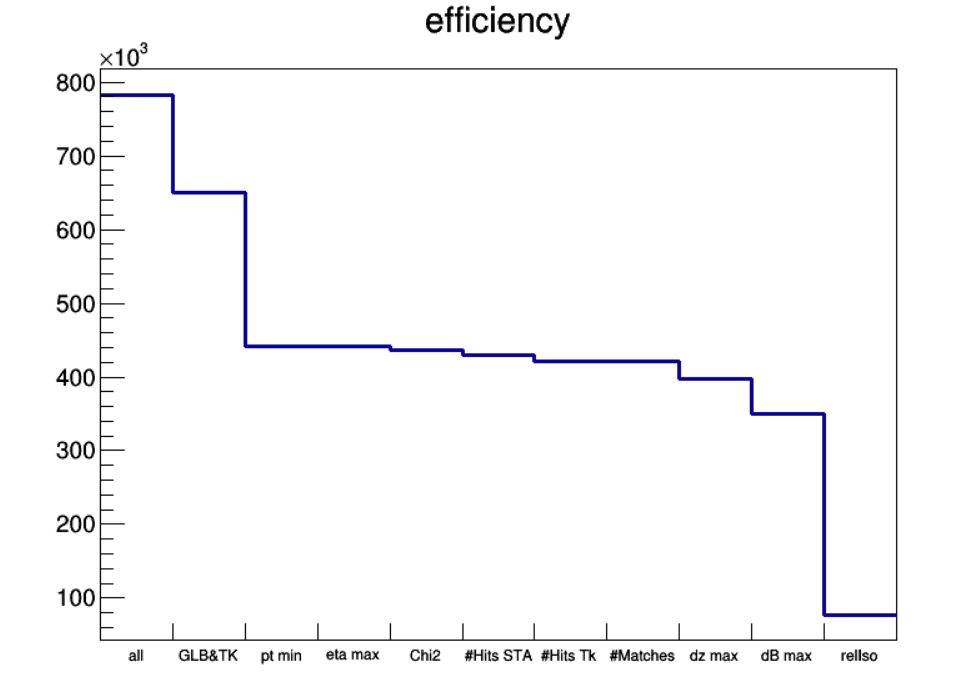
\includegraphics[scale=0.2]{efff.png}
					\caption{\label{Img:eff}Number of muons left after each filter}
				\end{figure}

			From the plot of the figure \ref{Img:eff}, the number of initial muons detected can be obtain (781606) as well as the number of final muons that pass all the filter (77745). With these values, the efficiency can be obtained, obtaining a total efficiency of 9.9\%.

			The invariant mass of the initial muons detected and the final muons after the filters are shown in Figure \ref{Img:invmass}. In this plot the equation \ref{eq:invariantMass} is used.

				\begin{figure}[H]
					\centering
					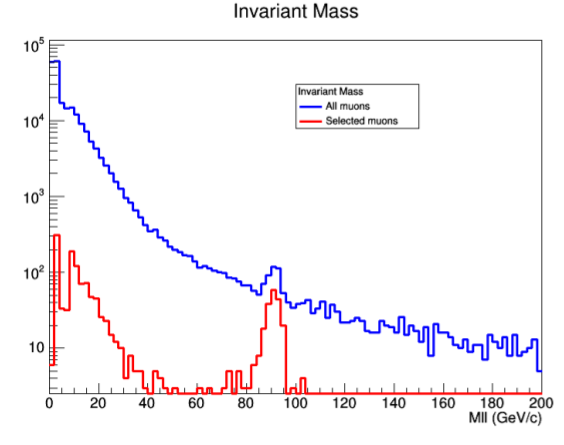
\includegraphics[scale=0.38]{invmass.png}
					\caption{\label{Img:invmass}The invariant mass of the initial muons detected and the final muons after the filters.}
				\end{figure}

			In Figure \ref{Img:invmass} there is a clearly peak at around 90 GeV that can be consider a good candidate to be the Z boson. Therefore, this peak is fit to a gaussian distribution in Figure \ref{Img:gassss} due to the detector resolution is relatively poor.

				\begin{figure}[H]
					\centering
					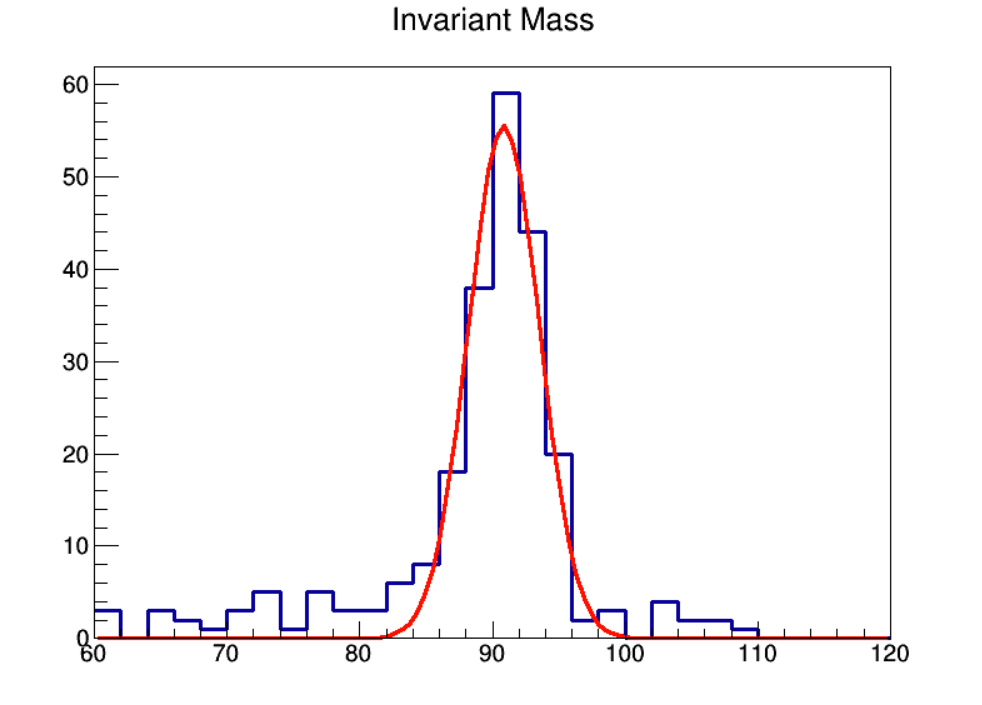
\includegraphics[scale=0.23]{gasss.png}
					\caption{\label{Img:gassss}The 90 Gev peak fit to a gaussian distribution.}
				\end{figure}

			Now, the Z$^0$ boson mass and decay width can be obatined from the plot of the figure \ref{Img:gassss}.

				\begin{equation}
					\begin{matrix}
						m_{Z^0} = ( 90.86 \pm 0.23 ) \; GeV/c^2
						\\
						\\
						\Gamma = ( 2.679 \pm 0.181 ) \; GeV/c^2
					\end{matrix}
				\end{equation}

		\section{Conclusion}

			The mass of the Z$^0$ boson has been obtained by the discrimination and analysis of the events obtained in the CMS detector, obtaining a value of $m_{Z^0} = ( 90.86 \pm 0.23 ) \; GeV/c^2$. The differences with the accepted value, of $( 91.1876 \pm 0.0021 ) GeV/c^2$, is just a 0.36\%. However, this value is not inside the error interval obtained. With the value obtained for the decay width occures the same, been the accepted value of $(2.4952 \pm 0.0023) GeV/c^2$, outside the error interval. However, the differences between the obtained value and the accepted is 7\%.

			The fact that the values obtained are so close to the accepted values but not in the error interval could be due to the fit made, been a Breit-Wigner function fit a more apropiate. There is also some background effects that could affect the final values.

	\end{multicols}

%----------------------------------------------------------------------------
%     APPENDIX
%----------------------------------------------------------------------------


	    		
%----------------------------------------------------------------------------
%     BIBLIOGRAPHY
%----------------------------------------------------------------------------

	%\bibliographystyle{unsrt}
	%\bibliography{biblio}

\end{document}


%----------------------------------------------------------------------------
%            TEMPLATES
%----------------------------------------------------------------------------

%----------------------------------------------------------------------------
%            how to insert an image
%----------------------------------------------------------------------------

%	\begin{figure}[H]
%		\centering
%		\includegraphics[scale= ]{nombre de la imagen.jpg}
%		\caption{\label{Img:widgets}el pie de pagina que le quieras 	poner a la imagen}
%	\end{figure}
 
%----------------------------------------------------------------------------
%            how to insert a table
%----------------------------------------------------------------------------

%	\begin{table}[H]
%		\centering
%		\begin{tabular}{|c|c|c|c|}
%			\hline
%			\centering
%				Altura(h) & Distancia (d) & Elaboracion (e) & Longitud (l) \\
%				($\pm0.5$ mm) & ($\pm0.5$ mm) & ($\pm0.5$ mm) & ($\pm0.5$ mm) \\ \hline
%				 &  &  &  \\ \hline
%				 &  &  &  \\ \hline
%				 &  &  &  \\ \hline
%				 &  &  &  \\ \hline
%				 &  &  &  \\ \hline
%		         &  &  &  \\ \hline
%		\end{tabular}
%		\caption{\label{Tab:widgets}pie de pagina que le quieras poner}
%	\end{table}

%----------------------------------------------------------------------------
%             How to remove the label in equactions
%----------------------------------------------------------------------------

%	\begin{equation*}
%		
%	\end{equation*}

%----------------------------------------------------------------------------
%              How to set bibliography
%----------------------------------------------------------------------------

%\bibliographystyle{unsrt}
%\bibliography{biblio}
%
%Then you have to set a .bib document such as the next template
%
%	@book{nickname,
%	author = {},
%	title = {},
%	edition = {},
%	year = {},
%	volume = {},
%	ISBN = {}
%	}
%
%	@ARTICLE{nickname,
%	author = {},
%	title = {},
%	year = {},
%	volume = {},
%	}


%----------------------------------------------------------------------------
%              END
%----------------------------------------------------------------------------
